%-------------------------------------------------------------------------------
% Copyright (c) 2015-2016 University of Luxembourg.
% All rights reserved. This program and the accompanying materials
% are made available under the terms of the Eclipse Public License v1.0
% which accompanies this distribution, and is available at
% http://www.eclipse.org/legal/epl-v10.html
% 
% Contributors:
%     Alfredo Capozucca - initial API and implementation
%     Benoit Ries - minor updates
%     Nicolas Guelfi - most content from messirbook
%-------------------------------------------------------------------------------
%%%%%%%%%%%%%%%%%%%%%%%%%%%%%%%%%%%%%%%%%%%%%%%%%%
\PassOptionsToPackage{usenames,svgnames,table}{xcolor}
\documentclass[graybox,envcountchap,sectrefs]{./../lu.uni.lassy.excalibur.standard.report.libraries/styles/svmono}  
%%%%%%%%%%%%%%%%%%%%%%%%%%%%%%%%%%%%%%%%%%%%%%%%%%
%%% DO NOT CHANGE THE ORDER
\usepackage{./../lu.uni.lassy.excalibur.standard.report.libraries/styles/style-messir-common}
\usepackage{./../lu.uni.lassy.excalibur.standard.report.libraries/styles/style-messir-report-post}
\usepackage{breakurl} 
\usepackage{graphicx}
%--------------------------------------------
  
% DOCUMENT BEGIN
%--------------------------------------------
\begin{document}
%-------------------------------------------------------------------------------
\newgeometry{textwidth=17cm,textheight=23.7cm} 
 
\input{./../lu.uni.lassy.excalibur.standard.report.libraries/defs/msr-def.tex}
% ***************************************
% test-case schema template
\newenvironment{lyxlist}[1]
  {\begin{list}{}
    {\settowidth{\labelwidth}{#1}
      \setlength{\leftmargin}{\labelwidth}
      \addtolength{\leftmargin}{\labelsep}
      \renewcommand{\makelabel}[1]{##1\hfil}}
      \setlength{\itemsep}{0ex}
      \addtolength{\baselineskip}{-5pt}
			\setlength{\parskip}{0pt}
			\setlength{\parsep}{0pt}}
  {\end{list}}
  
  
  \def\Remark{\noindent\textbf{Remark-}}
  
  \DeclareRobustCommand{\mysystemname}{\textbf{\textit{{\color{MediumPurple}MySystem
  (v1.0)}}}~}

\newglossaryentry{Glossary} 
{name={Glossary},
description={the description of terms that are
likely unfamiliar to the audience. The glossary shall include an alphabetical list of
terms and definitions. Documentation using abbreviations and acronyms unfamiliar
to the audience shall include a list with definitions, which may be integrated
with the glossary. Terms included in the glossary should also be defined on
their first appearance in printed documentation. Here there is an example of how
to include an expression into the glossary: \gls{socialware}. 
}, 
plural={Glossaries}
}



\newglossaryentry{Concept Model}
{name={Concept Model},
description={the Model that describes the different types required to specify
the software system.}, 
plural={Concept Models},
symbol={\msrglsstyle{Concept Model}}
}

\newglossaryentry{Environment Model} 
{name={Environment Model},
description={the Model that describes the different actors supposed to interact
with the software system.}, 
plural={Environment Models},
symbol={\msrglsstyle{Environment Model}}
}

\newglossaryentry{MVC} 
{name={Model-View-Controller},
description={the pattern followed to design the Graphical User Interfaces
of the software system.}, 
plural={Model-View-Controllers}, 
symbol={\msrglsstyle{Model-View-Controller}}
}


\newglossaryentry{Design Model} 
{name={Design Model},
description={The Design Class Model is composed of the contents of all design classes, i.e.
their (value) attributes and methods, all the navigable associations between
design classes, and the inheritance structure. The Design Class Model has to be
modelled as a UML Class Diagram.}, 
plural={Design Models}, 
symbol={\msrglsstyle{Design Model}}
}


\newglossaryentry{Interaction Model} 
{name={Interaction Model},
description={The Interaction Model shows how objects are expected to interact at run-time to
support the \emph{system operations} specified in the \emph{Operation Model}
made during the Analysis Phase. There must exist an \emph{Interaction Model} for
each system operation specified in the \emph{Operation Model}. An Interaction Model has to be
modelled as a UML Sequence Diagram.}, 
plural={Interaction Models}, 
symbol={\msrglsstyle{Interaction Model}}
}

\newglossaryentry{Deployment View} 
{name={Deployment View},
description={The physical view depicts the system from a system engineer's
point-of-view. It is concerned with the topology of software components on the
physical layer, as well as the physical connections between these components.
For example, how many nodes are used and what is deployed on what node. A
Deployment View is modelled as a UML Deployment Diagram.}, 
plural={Deployment Views}, 
symbol={\msrglsstyle{Deployment View}}
}


\newglossaryentry{Implementation View} 
{name={Implementation View},
description={This view describes the software system components. It focuses on
software modules and subsystems. It describes the hierarchies or layers for
components. This view is modelled as a UML Component Diagram.},
plural={Implementation Views}, 
symbol={\msrglsstyle{Implementation View}}
}


\newglossaryentry{Processing View} 
{name={Processing View},
description={This view deals with the dynamic aspects of the system. It is
aimed at describing processes taking part at runtime and, in particular, how
such process communicate among each other. A Processing View is modelled as a
UML Sequence Diagram.},
plural={Processing Views}, 
symbol={\msrglsstyle{Processing View}}
}


\newglossaryentry{Use-Case Instance View} 
{name={Use-Case Instance View},
description={The description of an architecture is illustrated using a small set
of use-case instances (or scenarios). The scenarios describe sequences of
interactions between objects, and between processes. They are used to identify
architectural elements and to illustrate and validate the architecture design.
They also serve as a starting point for tests of an architecture prototype. A
scenario has to be modelled as a UML Sequence Diagram.}, 
plural={Use-Case Instance Views}, 
symbol={\msrglsstyle{Use-Case Instance View}}
}

%  General Messir Glossary
\newglossaryentry{real number}
{name={Real number},
description={name of the set of real numbers.},
plural={reals},
symbol={\ensuremath{\mathbb{R}}}
}

\newglossaryentry{system operation}
{name={System Operation},
description={a functionality of the system that can be triggered by a message
sent by an actor belonging to the environment.}, plural={system operations},
symbol={\msrglsstyle{system operation}}
}

\newglossaryentry{societics}
{name={Societics},
description={Represents the fields of hardware/software
systems used for the society extension.}, 
symbol={\msrglsstyle{societics}}
}

\newglossaryentry{direct actor}
{name={Direct Actor},
description={an actor that interacts directly with the system. It thus belongs
to the environment.},
plural={direct actors},
symbol={\msrglsstyle{direct actor}}
}

\newglossaryentry{indirect actor}
{name={Indirect Actor},
description={an actor that interacts indirectly with the system through a direct
actor.  It thus belongs the domain but not to the environment.}, 
plural={indirect actors},
symbol={\msrglsstyle{indirect actor}}
}

\newglossaryentry{abstract actor}
{name={Abstract Actor},
description={an actor that does not exist in real life.},
plural={abstract actors},
symbol={\msrglsstyle{abstract actor}}
}

\newglossaryentry{socext}
{name={Society extension},
description={The society obtained by grouping people using natural means
extended with artificial means.},
symbol={\msrglsstyle{societics}}
}

\newglossaryentry{usecase}
{name={Use case},
description={A use case describes a sequence of actions that provide something
of measurable value to an actor. and is drawn as a horizontal ellipse.},
plural={Use cases}, 
symbol={\msrglsstyle{Use case}} 
}

\newglossaryentry{Ph-Meter}
{name={Ph-Meter},
description={A Ph-Meter is a instrument which measures acidty on a scale of 1
to 12 where 12 is alkaline.}, plural={Ph-Meters},
symbol={\msrglsstyle{Ph-Meter}}
}
\newglossaryentry{EC-Meter}
{name={EC-Meter},
description={An EC-Meter is a instrument which measures the nutrient level in
the soil or in a liquid.}, plural={EC-Meters}, symbol={\msrglsstyle{EC-Meter}}
}
\newglossaryentry{VGA}
{name={VGA},
description={VGA is an input format to display the software from the computer
on the screen.}, plural={VGA's}, symbol={\msrglsstyle{VGA}} }

\newglossaryentry{crisis}
{name={crisis},
description={A crisis is an alert for example when sompthing not usual is
happening like an illegal intrusion.}, plural={crisises},
symbol={\msrglsstyle{crisis}} }

\newglossaryentry{actor}
{name={Actor},
description={An actor is a person, organization, or external system that plays a
role in one or more interactions with the system.},
plural={actors},
symbol={\msrglsstyle{actor}}
}
\newglossaryentry{socialware}
{name={Societics},
description={Represents the fields of hardware/software
systems used for the society extension.},
symbol={\msrglsstyle{Societics}}
}

% \newglossaryentry{}
% {name={\msrglsstyle{}},
% description={},
% symbol={\msrglsstyle{actor}} }
 

%TITLE
%******************************************

\title{
\begin{tabular}{|>{\centering\arraybackslash\hspace{0pt}}p{16cm}|}
\hline
\textbf{\mysystemname}\\ \\
	\textbf{\msrmessir User Manual}\\
	\textbf{ - v 1.0.3 - }\\
	\textbf{\large Based on IEEE Std 1063-2001 \cite{IEEE-2001-userdocumentation}}\\
\hline 
\end{tabular}
\vspace{2cm}}
 
%******************************************
\author{
\begin{tabular}{l}
		Schroeder Lionel author 1\\
		Mayer Mark author 2\\
		Jérôme Bortuzzo author 3\\
		\\Greenhouse\\
\end{tabular}}

\date{\today~-~\currenttime}
%****************************************************


\maketitle
\newpage

%TOC
\setcounter{tocdepth}{2}
\addtocounter{secnumdepth}{2}
\tableofcontents
\newpage

%TOF
\listoffigures
\newpage

% No requiered by the standard
%TOL
%\lstlistoflistings
%\newpage

%DOCUMENT STRUCTURE

% General Information
\chapter{Product information}
%Reducing the spacing from the title
\vspace{-6em}


\section{Identification}
Greenhouse is a tool that allows you to grow different plants in an efficient
way. The software allows you to monitor the different data acquisition
sensorsHeloo world on the screen.\hfill\break


\begin{table}
\begin{center}
\label{tab:Sensors}
\begin{tabular}{| m{3cm} | m{4cm} |}
\hline
\textbf{Sensor name} & \textbf{Sensor id} \\ \hline 
Temperature & TemperatureSensorXX \\ \hline 
Humidity & HumiditySensorXX \\ \hline 
Light & HumiditySensorXX \\ \hline 
Motion & MotionSensorXX \\ 
\hline 
\end{tabular}
\end{center}
\end{table}
\begin{table}
\begin{center}
\label{tab:Sensors}
\begin{tabular}{| m{4cm} | m{4cm} |}
\hline
\textbf{Other Parts} & \textbf{ID} \\ \hline 
Security Camera & SecurityCameraXX \\ \hline 
\textbf{\emph{\glspl{EC-Meter}}} & ECMeterXX \\ \hline 
\textbf{\emph{\glspl{Ph-Meter}}} & PhMeterXX \\ \hline 
Computer & ComputerXX \\ \hline
Hard-disk & HardiskXX \\ 
\hline 
\end{tabular}
\end{center}
\end{table}
\hfill\break
The computer runs the operating system Windows 10 Pro edition on the current
version 1703. An mouse and keyboard and a display of 24 inches are also
connected to the computer. Keyboard and mouse via cable USB and the display via
\textbf{\emph{\glspl{VGA}}}. \hfill \break\break
The storage for the different datas are stored on three different hard-drives of
the company Seagate Barracuda. Two hard-drive of 512 gb for the digital storage
of the amount of crops and one for sensors data. The third one is for the video
recording of the size of 1 tb. The hard-drives are connected to the mainboard of
the computer with a Sata 3 cable for the communication. The Model Number is
ST100DM010.\hfill \break\break
Inside the greenhouse:\hfill \break\break
Two temperature sensors are set up in each room. Monnit Wi-Fi Temperature
Sensors which telecommunicate over wifi. It takes Batteries as energy
source. In addition the item number is MN-2-WF-TS-ST.\hfill \break\break
The humidity sensor are also placed inside the big pots every square meter one. 
The Wemos Higrow ESP32 is used here to measure the humidity in the soil. The
telecommunication is over wifi and Batteries are used as power source.\hfill
\break\break
The light sensors are also inside the greenhouse every square meter one.\hfill
\break\break
The motion sensors are positioned on every corner of each room. The supported
motion sensor is the Philips Hue Motion sensor which power Source are batteries
and detects a person on a range of 5 meter. The motion sensors are connected via
wireless,in addition the motion detection range is 100 degrees. The product
number is 464602.\hfill \break\break
The security camera is inside the greenhouse one in each room and on the roof.
The camera is from SV3C it can record up to 15 fps on resolution of 2592x1944
and it is waterproofed. The view angle is 80 degrees an and the connection of
the ethernet is wired. The support of video compression H.265 is also
possible.\hfill \break\break
The EC-Meter is positioned inside the water tank.\hfill \break\break
The ph meter is positioned inside the soil to read ph scale of the soil where
the plants are and to check the ph scale inside the water tank.\hfill
\break\break



\section{Copyright}
All content on the website including but not limited to  the logo of the
greenhouse the design  and the functions of the software are copyright.
Copyright © 2017 by Greenhouse All Rights Reserved. protected.

\section{Trademark notices}
The Greenhouse logo, name and software design are part of the Greenhouse
trademark. It is strictly prohibited to use anything that could be mistaken for
a Greenhouse product. Anything that influences the income of greenhouse
negatively or impacts the name of Greenhouse in a bad way. Artwork ,designs and
imagery are trademarks or copyrighted material of the Greenhouse.


\section{Restrictions}
All rights reserved. The software is licensed to the client, no part of this
software or its documentation shall be reproduced, redistributed in any from,
including taking pictures, screenshots, recording and any other electroni
methods  without the EXCLUSIVE permission from Greenhouse. The only exception is
in the case of a review of the software in a non commercial way or in the case
of educational use, it is allowed to share the experience of the project and to
criticize it.  In case of a request for a permission contact the support office
of the greenhouse at support@greenhouse.com. This product produced by MBSA Co.
allows you to operate a SPCG. The goal of this products use is to maximize crop harvest and to maintain a SPCG. The product is not meant for other uses than gardening otherwise all warranty and support will be canceled and we will not take any responsibilities towards the product.

The Software will always be our intellectual property. You are not allowed to
sell nor to copy and sell the product (including software and hardware). This is
a standalone system drafted by MBSA Co..

\section{Warranties}
Greenhouse has a for 30 days return policy. The software is covered under
warranty for one year. The warranty covers all the functionality of the software
that it executes the different actions appropriately.
Every hardware warranty will be claimed by the company who produced them.  See
the table below for the warranties of the different items.

\begin{table}
\begin{center}
\label{tab:Warrenties}
\begin{tabular}{| m{4cm} | m{4cm} | m{4cm} |}
\hline
\textbf{Manufractuer} & \textbf{Name} & \textbf{Warrentie} \\ \hline 
Seagate Barracuda & Hard-Disk & 2 Years \\ \hline 
Philps Hue & Motion Sensor & 2 Years \\ \hline 
SV3C & Security Camera & 2 Years \\ \hline 
Wemos Higrow ESP32 & Humidity Sensor & 180 Days \\ \hline
Monnit Wi-Fi & Temperature Sensor & 1 Year \\ \hline
??? & Ph-Meter & ? Year \\ \hline
??? & Ec-Meter & ? Year \\ 
\hline 
\end{tabular}
\end{center}
\end{table}
\hfill\break

\section{Contractual obligations}
The client can only use the software for one specific project or enterprise. The
software must be installed by Greenhouse certified technicians. If the client
encounters any problems with the software Greenhouse will provide support from
certified technicians. The client is not allowed to seek support from any third
party. The computer provided is only intended for use with the software provided
by Greenhouse. The client is not allowed to install any other software or use
the computer for any other purpose. In case there is a faulty sensors the client
has to contact Greenhouse to either outright replace the sensors or to give
instructions to the client on how to repair the sensor.

\section{Disclaimers}
A refund for the software is only possible in the first 30 days after receiving
the software. Greenhouse is not responsible for any damages that occur during
unspecified use of our software. In addition Greenhouse is not responsible of
any hardware failure nor is Greenhouse responsible for any data lost in that
event, we will redirect you to the company which produced the hardware to
request warranties. Also in a case of software failure we can not be hold
responsible if any plants get harmed. Greenhouse is not responsible for any
damage done by third parties who gained unauthorized access to the software or
the webpage. Greenhouse is not responsible for any bodily or psychological harm
caused by unspecified use of the software. In case that the client modifies the
software himself the warranty for the software will be null and void. In case of
damage during a repair on a sensors Greenhouse is not responsible if the clients
technician failed to fully comply with our instructions.

\section{Contact}
Greenhouse\break
1234 Resistance avenue \hfill \break
Bascharage L - 4942\hfill \break
www.greenhouse.lu\hfill \break
It is possible to contact us via email: support@greenhouse.com or via phone: 1-800-GREENHOUSE 


\newpage

% Introduction
\chapter{Introduction}
\label{chap:introduction}

\section{Scope}

This user manual will explain you how to use our software efficiently. It will
show you how the different sensors interact with each other and how statistics
are used to schedule tasks. It will also show you how you can properly interact
with the software. It will be useful reference material during the use of the
Software. This document will not show you how to integrate the software in your
specific environment. Thus not showing you how to create and implement databases
nor does it show you how to care for the different plants. This document wills
also not show you how to properly install the sensors.


\section{Purpose}

This document defines all essential information for the user to use the software application. 
The system functions are shown step by step for the user. In case of a
\textbf{\emph{\glspl{crisis}}} the user can look up in this file with the
given error code which action has to be taken accordingly.
In addition the definition of different icons will be shown and explained.


\section{Intended audience}

The software is intended to be primarily used in the enterprise sector more
specially the agriculture sector. The manual  will help the people concerned
with operating the software correctly. The gardener can use this document to
understand how he can interact with the system and retrieve information about
the inventory. The manager can learn how to add tasks to the schedule correctly,
how to access camera. The technician will know where to look for problems with
the sensors as well as what alerts he can expect. The gardener and the
technician can find information about the schedule and what task can be given to
the respecting personnel.

\section{\mysystemname}

The software is used in agriculture/gardening that means planting and harvesting
plants. The main purpose is to do so in the most efficient way by using
different hardware like sensors. Basically the software allows the user to check
if the soil needs nutrition or water to allow for a optimal growing of the
plants. Also the software gives tasks to the gardner so that no mistakes are
made by the individual human. The software creates statistics with the data
gather by the sensors about the plants and their environment. The software gives
insight to the results achieved with varying environmental conditions.


\subsection{Actors \& Functionalities}

The \textbf{gardener} is in charge of planting and retrieving the plants and
updating the storage if any crops are used. He also gets notified if any plant
needs water or additional minerals in the soil. The gardner uses other actors
like the ph meter and the ec meter to check the water.\break

\noindent The \textbf{technician} observes if any sensors are damaged or must be
recalibrated. He gets notified if any sensor is defect or the environmental
system has crashed to reboot it.The technician can request more sensors.\break

\noindent The \textbf{manager} keeps track of the storage of crops. If the
storage is depleting, he calls the delivery firm to buy more. In case of a crisis that
means by intrusion or natural damage like fire he will be alerted and can then,
if necessary, call the emergency services.\break

\noindent The \textbf{director} gets a report every month which consists of how
many crops have been used, how many plants were harvested or have been removed. In a case
of a crisis the director also gets automatically notified like the
manager.\break

\noindent The non human Actors:\hfill \break
The \textbf{temperature sensor} is in charge to read the temperature and to
communicate the data to the computer.

\noindent The \textbf{humidity sensor} is in charge to collect the humidity
percentage in the soil and communicate it to the computer.

\noindent The \textbf{light sensor} is in charge to collect the light density
 inside and outside the greenhouse and to communicate the data to the
 computer.

\noindent The \textbf{motion sensor} is  in charge of the security of the
greenhouse. The sensors captures any motion by human or inhuman to the
computer.


\noindent The \textbf{ph meter} is used to check if the water has the perfect ph
scale for the plants and has to communicate the data to the computer.

\noindent The \textbf{Ec meter} is in charge the check if the nutrition inside
the water tank is good.

\noindent The \textbf{security camera} is recording what is happening inside the
greenhouse which is displayed in live on the website.

\noindent The mouse and keyboard are used to control and give input to the
computer and the web page.

\noindent The display is there to display the data webside and so on. 

\noindent The heater is used to warm up the different rooms to a given
temperature.

\noindent The windows can automatically be opened to give fresh air and cool
down the temperature.


\subsection{Operating environment}
Brief overview of the infrastructure on which the software is deployed and used.
Controlling part of the software will run on a windows 10 Pro environment while
created statistics will be stored in a SQL database. Data from the sensors will
also be stored in a SQL database. The website can be accessed from a
phone/tablet or computer. Windows 10 is used for its GUI so it is easier to use
for the people using the software.

\section{Document structure}  
Information on how this document is organised and it is expected to be
used. Recommendations on which members of the audience
should consult which sections of the document, and explanations about the used
notation (i.e. description of formats and conventions) must also be provided.

\newpage

% User guide

\chapter{Usage Guide}

\label{chap:usage_guide}



This section is aimed at describing the general use of the software, since it is
\textbf{deployed, configured} and \textbf{run}.

This software is used by actors. These actors rely on the software to perform a
set of business activities (called here procedures) aimed at reaching a
particular goal. 

These prodedures are splet in two groups:
\begin{itemize}
  \item \textbf{Multi-procedures:} which are procedures at \textbf{summary} or
  \textbf{user-goal} level involving several active or pro-active actors.
  Each of these procedures aims at illustrating intertwined
  business activities required to be performed by the involved actors
  to reach the expected goal. Each business activity between the system and an
  actor must correspond to a \textbf{system operation} instance given with actual parameter values.

  \item \textbf{Mono-procedures:} which are procedures at \textbf{summary} or
  \textbf{user-goal} level involving only one active or pro-active actor.
  Each of these procedures aims at illustrating the required business
  activities an actor has to perform to reach the expected goal. Each business
  activity between the system and the actor must correspond to a \textbf{system
  operation} instance given with actual parameter values.

\end{itemize}



Each process has to be documented using the following textual description
template \cite{armour01usecase} \textbf{BUT its content must be as low level as possible with actual values}:

\vspace{0.5cm}

\hrule
\begin{lyxlist}{PC1}

\small{

\item [\textbf{Procedure:}] ProcessMissionOne
\item [\textbf{Scope:}] Crisis Management System (\emph{CMS})
\item [\textbf{Primary Actor}:] Coordinator John
\item [\textbf{Secondary Actor(s)}:] FirstAidWorker Bob,\\
                  ExternalResourceSystem ERS
\item [\textbf{Goal:}] The intention of the Coordinator is to process mission
with ID equal to 1.
\item [\textbf{Level}:] User-goal level
\item [\textbf{Main~Success~Scenario}]:\\
1. \emph{John} instructs the \emph{CMS} to process the mission with ID equal to 12.031005\\
2. \emph{CMS} selects the internal worker \emph{Bob} to execute the mission 12.031005\\
3. \emph{CMS} instructs \emph{Bob} to behave as \emph{First Aid Worker (FAW)}\\
4. \emph{Bob} informs the \emph{CMS} of his arrival\\
5. \emph{Bob} informs the \emph{CMS} that he starts to execute the mission 12.031005\\
6. \emph{Bob} informs the \emph{CMS} that the mission 12.031005 outcome is ``Mission completed''


\item [\textbf{Extensions}]:\\
2.a None internal worker can execute the mission\\
\hspace*{0.5cm} 2.a.1 \emph{CMS} sends a request for an external resource to the \emph{ERS} actor instance\\
\hspace*{0.5cm} 2.a.2 \emph{ERS} informs \emph{CMS} that the request can be processed\\
\hspace*{0.5cm} 2.a.3 \emph{ERS} informs \emph{CMS} that \emph{Bob} can now be selected as first aid worker\\
\hspace*{0.5cm} \textbf{procedure continues at step 3}

}

\end{lyxlist}
\hrule
\vspace{0.5cm}




\Remark{Processes presentation}: processes should be introduced to the
reader in a pedagogical manner. Thus, simple and common processes should be presented before
than more complex and less utilised ones.

\Remark{Graphical User Interfaces (GUIs)}: include GUIs screenshots to show the
different stages of the process while its is performed by the actor(s).






\section{Multi-procedures}

\subsection{Ask for new sensor}

\vspace{0.5cm}
\hrule
\hfill \break
\begin{lyxlist}{PC1}
\small{
\item [\textbf{Procedure:}] AskForNewSensor
\item [\textbf{Scope:}] New Sensor demand to the manager.
\item [\textbf{Primary Actor}:] Technician
\item [\textbf{Secondary Actor(s)}:] Manager
\item [\textbf{Goal:}] The intention that the technician can ask a new Sensor to
the manager and to show to the manager the demand.
\item [\textbf{Level}:] User-goal level
\item [\textbf{Main~Success~Scenario}]:\\
1. \emph{Gardner} complets the diffrent text fields with there given
information and presses the button \emph{push to the manager}. 
\begin{figure}
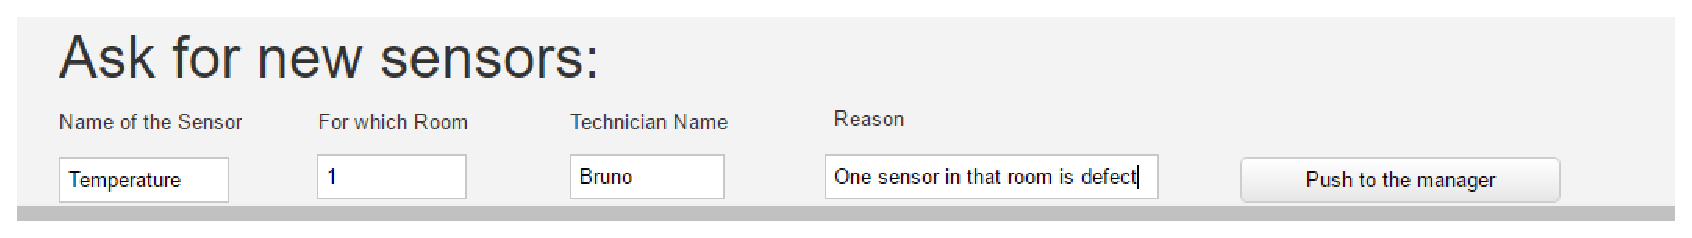
\includegraphics[width=1\textwidth]{images/AskForSensor.eps}
\end{figure} \\
2. \emph{System} pushes the information to the Manager Sensor Table on the
 managerscreen. \\
 \begin{figure}
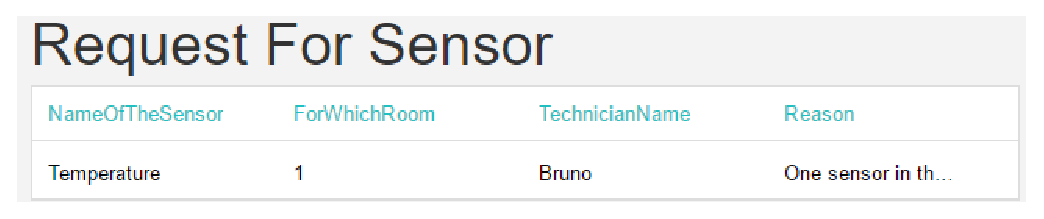
\includegraphics[width=1\textwidth]{images/requestsensor.eps}
\end{figure}
3. \emph{System.NoTA} alerts \emph{Manger} that a request has been send from
the \emph{Gardner}.\\
4. \emph{Manager} can contact now the company of the asked sensor for a new
one.\\
\item [\textbf{Extensions}]:\\
2.a  \emph{Manager} sends to the Gardner a message of
validation or not.\\
}
\end{lyxlist}

\hrule
\vspace{0.5cm}


\subsection{Sign In}
\vspace{0.5cm}
\hrule
\hfill \break
\begin{lyxlist}{PC2}
\small{
\item [\textbf{Procedure:}] SignIn
\item [\textbf{Scope:}] Identified usage of the software
\item [\textbf{Primary Actor}:] User
\item [\textbf{Secondary Actor(s)}:] Greenhouse Software GS
\item [\textbf{Goal:}] Show the user GUI to manage the garden
\item [\textbf{Level}:] User-goal level
\item [\textbf{Main~Success~Scenario}]:\\
1. \emph{User} enters a username and password combination and signs in\\
2. \emph{GS} looks up the user rights defined by the administrator\\
3. \emph{GS} now show the correct Graphical User Interface (GUI) \emph{(Gardener, Technician, Manager or Administrator)} able to control the garden.
\item [\textbf{Extensions}]:\\
1.a Wrong username and password combination\\
\hspace*{0.5cm} 1.a.1 \emph{GS} notifies the \emph{User} that the entered information are wrong\\
\hspace*{0.5cm} \textbf{procedure recontinues at step 1}
}
\end{lyxlist}
\hrule
\vspace{0.5cm}



\subsection{Adding data}
\vspace{0.5cm}
\hfill \break
\hrule
\begin{lyxlist}{PC3}
\small{
\item [\textbf{Procedure:}] Adding data
\item [\textbf{Scope:}] Adding data to a datalist
\item [\textbf{Primary Actor}:] Manager
\item [\textbf{Secondary Actor(s)}:] Greenhouse Software GS
\item [\textbf{Goal:}] Adding a task to the schedule
\item [\textbf{Level}:] User-goal level
\item [\textbf{Main~Success~Scenario}]:\\
1. \emph{User} presses the “add” button\\
2. \emph{GS} adds the task to the schedule\\
}
\end{lyxlist}
\hrule
\vspace{0.5cm}








\section{Mono-procedures}
Mono-procedures must be grouped by actors.


\subsection{MyActor1}

\subsubsection{MyProcedure1MyActor1}
\ldots

\subsubsection{MyProcedure2MyActor1}
\ldots


\subsection{My-Actor2}

\subsubsection{MyProcedure1MyActor2}
\ldots

\subsubsection{MyProcedure2MyActor2}
\ldots















\newpage

% Software operations
\input{doc/software-operations/software-operations.tex}
\newpage
  
% Error messages and problem resolution
\input{doc/error-messages/error-messages.tex}
\newpage

%APPENDICES
\appendix
\input{doc/appendix/appendix.tex}
\newpage
 
    
%GLOSSARY
%Uncomment the line below if you want to print all glossaries no matter if they
% appear in the document
%\glsaddall
\printglossaries
\newpage


%BIBLIOGRAPHY
\cleardoublepage 
\bibliographystyle{./../lu.uni.lassy.excalibur.standard.report.libraries/styles/lncs} 
\bibliography{./../lu.uni.lassy.excalibur.standard.report.libraries/defs/references/messir,doc/bibliography/user-manual}
\label{sec:references}

 
\end{document}
